\documentclass{article}

\usepackage{josuamathheader}
\usepackage{tikz}
\usepackage{pgfplots}

\newcommand{\diam}{\operatorname{diam}}
\begin{document}
\def\headheight{25pt}
\analayout{3}
    \section*{Aufgabe 1}    
    Sei $\mathscr{K}$ die Menge aller Mengen, die (1.1) erfüllen.
    Sei $U$ eine offene Menge. Wir definieren die Folge abgeschlossener Mengen 
    \[A_n = \{x \in U\colon d(x, U^c) \geq \frac{1}{n}\} \subset U.\]
    Da zu jedem $x \in U$ ein $N \in \N$ existiert mit $U_{\frac{1}{n}}(x) \subset U$, ist dieses $x$ $\forall n \geq N$ in der Menge $A_n$ enthalten. Daraus folgt $A_n \nearrow U$ und damit $\mu(A_n) \nearrow \mu(U)$. Außerdem ist $U$ die inklusionsminimale offene Menge, die $U$ enthält. Daher sind alle offenen Mengen in $\mathscr K$ enthalten. Insbesondere sind also auch $\emptyset$ und $X$ enthalten. 
    Wir betrachten nun den Fall $\mu$ $\sigma$-endlich, aber nicht endlich. 
    Sei dafür $B \in \mathscr K$ mit $\mu(B)$ endlich. Dann darf $\mu(B^c)$ nicht endlich sein, da sonst $\mu(X) = \mu(B) + \mu(B^c) < \infty$ wäre. 
    
    Für $M = \{U \in \mathscr B(\R) \colon U \supset B, \text{offen}\}$ gilt $\inf \{\mu(U) | U \subset M\} = \mu(B)$. Es existiert daher eine Folge von offenen Mengen $(U_n)_{n\in\N} \in M$ mit $U_n \searrow B$.
    Wir betrachten die Folge $(U_n^c)_{n\in\N}$. Es gilt $U_n^c \subset B^c \forall n \in \N$, wobei $U_n^c$ abgeschlossen ist.
    Gilt $U_n \searrow B$, so folgt $U_n^c \nearrow B^c$. Daher gilt $\sup \{\mu(U^c) | U \in M\} \geq \mu(B^c)$. Da aber $U_n^c \subset B^c$ folgt aus der Monotonie des Maßes $\mu(U_n^c) \leq \mu(B^c)$ und damit $\mu(B^c) = \sup \{\mu(U^c) | U\in M\} = \sup \{\mu(U) | U \subset B^c, \text{abgeschlossen}\}$.

    Für $M = \{U \in \mathscr B(\R) \colon U \subset B, \text{abgeschlossen}\}$ gilt $\sup \{\mu(U) | U \subset M\} = \mu(B)$. Es existiert daher eine Folge von offenen Mengen $(U_n)_{n\in\N} \in M$ mit $U_n \nearrow B$.
    Wir betrachten die Folge $(U_n^c)_{n\in\N}$. Es gilt $U_n^c \supset B^c \forall n \in \N$, wobei $U_n^c$ offen ist.
    Gilt $U_n \nearrow B$, so folgt $U_n^c \searrow B^c$. Daher gilt $\inf \{\mu(U^c) | U \in M\} \leq \mu(B^c)$. Da aber $U_n^c \supset B^c$ folgt aus der Monotonie des Maßes $\mu(U_n^c) \geq \mu(B^c)$ und damit $\mu(B^c) = \inf \{\mu(U^c) | U\in M\} = \inf \{\mu(U) | U \subset B^c, \text{offen}\}$.
    
    Insgesamt erhalten wir $\mu(B^c) = \sup \{\mu(U) | U \subset B^c, \text{abgeschlossen}\} = \inf \{\mu(U) | U \subset B^c, \text{offen}\}$ und damit $B^c \in \mathscr K$.

    Sei nun $\forall n \in \N\colon B_n\in \mathscr K$. Dann gibt es zu $\epsilon > 0$ abgeschlossene Mengen $A_n$ und offene Mengen $U_n$ mit $A_n \subset B_n \subset U_n$ und $\mu(U_n \setminus A_n) \leq \frac{\epsilon}{2^{n+1}}$. Wir definieren $S \coloneqq \bigcup_{n\in \N} A_n$ und $U \coloneqq \bigcup_{n\in \N} U_n$. Dann gilt $S \subset \bigcup_{n\in \N} B_n \subset U$ und $\mu(U\setminus S)  \le \sum_{n = 1}^{\infty} \mu(U_n\setminus A_n) \leq \sum_{n = 1}^{\infty} \frac{\epsilon}{2^{n+1}} = \epsilon$. Die Menge $U$ ist offen, die Menge $S$ im Allgemeinen aber nicht abgeschlossen. Allerdings sind die Mengen $S^k \coloneqq \bigcup_{n=1}^k A_n$ abgeschlossen und es gilt $\mu(S^n) \nearrow \mu(S)$. Daher existiert ein $N\in \N$ mit $\mu(S^N) \geq \mu(S) - \epsilon$. Mit der Wahl $A \coloneqq S^N$ erhalten wir also $A \subset \bigcup_{n\in \N} B_n \subset U$ und $\mu(U\setminus A) \leq 2\epsilon$. Daraus folgt für $\epsilon \searrow 0$ die Aussage $\mu\left(\bigcup_{n\in \N} B_n\right) = \sup \left\{\mu(U) | U \subset \bigcup_{n\in \N} B_n, \text{abgeschlossen}\right\} = \inf \left\{\mu(U) | U \subset \bigcup_{n\in \N} B_n, \text{offen}\right\}$
    \section*{Aufgabe 2}
    \begin{enumerate}[(a)]
        \item Es gilt für $\delta = \frac{1}{n}$.
        \begin{align*}
            \mathscr H^s_\delta([0,1]) &= \inf \left\{\sum_{j \in \N} \diam(B_j)^s \colon [0,1] \subset \bigcup_{j\in \N} B_j, \diam(B_j) \leq \delta \right\}\\
            \intertext{$B_j = ([\frac{j-1}{n}, \frac{j}{n}])$ für $1 \leq j \leq n$ stellt eine Überdeckung von $[0,1]$ dar mit $\diam(B_j) \leq \frac{1}{n}$}
            &\leq \sum_{j = 1}^{n} \diam([\frac{j-1}{n}, \frac{j}{n}])^s\\
            &= n \cdot \left(\frac{1}{n}\right)^s\\
            &= n^{1-s}
        \end{align*}
        Es gilt nun $\mathscr H^s([0,1]) = \lim\limits_{n \to \infty} \mathscr H^s_{\frac{1}{n}}([0,1]) = \lim\limits_{n \to \infty} n^{1-s} = 0$ für $s > 1$.
        Aufgrund der Translationsinvarianz, Subadditivität und Monotonie von $\mathscr H^s$ gilt also $\mathscr H^s(A) = 0 \forall A \subset \R$.
        \item Sei $A \subset \bigcup_{j\in \N} B_j$ mit $\diam (B_j) \leq \delta$. Wegen $H^{s^*}(A) < \infty$ existieren Familien $(B_j)_{j\in \N}$ mit $\sum_{j \in \N} \diam(B_j)^{s^*} < \infty$. Wir betrachten also eine solche Familie $(B_j)_{j\in \N}$. 
        Es gilt dann für $s = s^* + \epsilon,\; \epsilon > 0$
        \[
            \sum_{j \in \N} \diam(B_j)^s = \sum_{j \in \N} \diam(B_j)^{(s^* + \epsilon)} \leq \sum_{j \in \N} \diam(B_j)^s \cdot \delta ^\epsilon  = \delta^\epsilon \cdot \sum_{j \in \N} \diam(B_j)^s.
        \]
        Für $\delta \to 0$ gilt dann also 
        \[
            \lim\limits_{\delta \to 0} \underbrace{\delta^\epsilon}_{\to 0} \cdot \underbrace{\sum_{j \in \N} \diam(B_j)^s}_{< \infty} = 0
        \]
        und damit $\mathscr H^s(A) = 0$.
        \item Sei $A \subset \bigcup_{j\in \N} B_j$ mit $\diam (B_j) \leq \delta$. Wegen $H^{s^*}(A) > 0$ existieren Familien $(B_j)_{j\in \N}$ mit $\sum_{j \in \N} \diam(B_j)^{s^*} > 0$. Wir betrachten also eine solche Familie $(B_j)_{j\in \N}$. 
        Es gilt dann für $s = s^* - \epsilon,\; \epsilon > 0$
        \[
            \sum_{j \in \N} \diam(B_j)^s = \sum_{j \in \N} \diam(B_j)^{(s^* - \epsilon)} \geq \sum_{j \in \N} \diam(B_j)^s \cdot \delta ^{-\epsilon}  = \delta^{-\epsilon} \cdot \sum_{j \in \N} \diam(B_j)^s.
        \]
        Für $\delta \to 0$ gilt dann also 
        \[
            \lim\limits_{\delta \to 0} \underbrace{\delta^\epsilon}_{\to \infty} \cdot \underbrace{\sum_{j \in \N} \diam(B_j)^s}_{>0} = \infty
        \]
        und damit $\mathscr H^s(A) = \infty$.
        \item Abzählbares $A = \{x_1,\dots, \}$ kann dargestellt werden als $A = \bigcup_{j\in \N} \{x_j\}$. Dabei ist $\diam(\{x_j\}) ^s = 0^s \overset{s > 0}{=} 0$ und damit $\sum_{j \in \N} \diam(B_j)^s = \sum_{j \in \N} 0 = 0$, also $\mathscr H^s(A) = 0 \forall s > 0$ und daher $\dim A = 0$.
        \item Wir können $A$ schreiben als Vereinigung von offenen Intervallen. Da jedes offene Intervall eine rationale Zahl enthält, ist die Vereinigung Insbesondere abzählbar. Für jede Überdeckung $(C_i)_{i\in \N}$ eines Intervalls $(a,b)$ gilt
        \[
            \sum_{i \in \N} \diam(C_i) \geq b-a > 0.
        \] (Der Beweis hierfür erfolgt analog zu $\sum_{i\in \N}) \diam(C_i) \geq 1$ für $(C_i)_{i\in \N}$ mit $[0,1] \subset \bigcup_{i\in \N} C_i$.)
        Insbesondere gilt also aufgrund der Monotonie von $\mathscr H^s$ $\mathscr H^1(A) \geq b-a > 0$. Wegen $\mathscr H^s (A) = 0 \forall s > 1$ gilt daher \[\dim A = \inf \{s \geq 0 \colon \mathscr H^s(A) = 0\} = 1.\]
    \end{enumerate}
    \section*{Aufgabe 3}
    \begin{figure}
        \centering
        % This file was created by tikzplotlib v0.9.4.
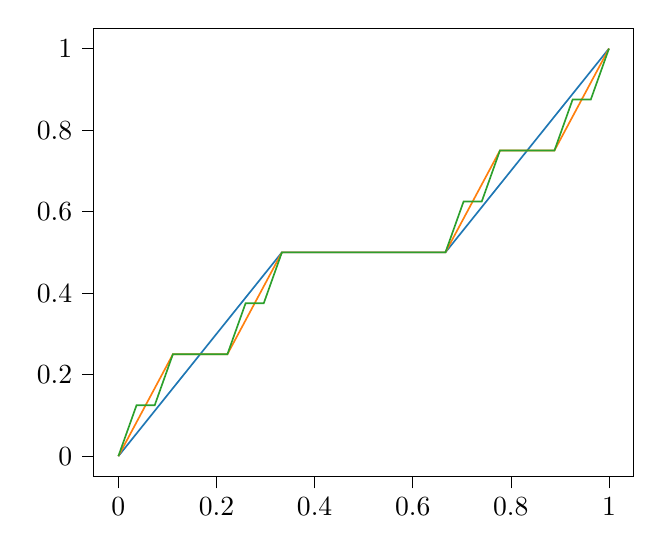
\begin{tikzpicture}

\definecolor{color0}{rgb}{0.12156862745098,0.466666666666667,0.705882352941177}
\definecolor{color1}{rgb}{1,0.498039215686275,0.0549019607843137}
\definecolor{color2}{rgb}{0.172549019607843,0.627450980392157,0.172549019607843}

\begin{axis}[
tick align=outside,
tick pos=left,
x grid style={white!69.0196078431373!black},
xmin=-0.05, xmax=1.05,
xtick style={color=black},
y grid style={white!69.0196078431373!black},
ymin=-0.05, ymax=1.05,
ytick style={color=black}
]
\addplot [semithick, color0]
table {%
0 0
0.333333333333333 0.5
0.666666666666667 0.5
1 1
};
\addplot [semithick, color1]
table {%
0 0
0.111111111111111 0.25
0.222222222222222 0.25
0.333333333333333 0.5
0.444444444444444 0.5
0.555555555555556 0.5
0.666666666666667 0.5
0.777777777777778 0.75
0.888888888888889 0.75
1 1
};
\addplot [semithick, color2]
table {%
0 0
0.037037037037037 0.125
0.0740740740740741 0.125
0.111111111111111 0.25
0.148148148148148 0.25
0.185185185185185 0.25
0.222222222222222 0.25
0.259259259259259 0.375
0.296296296296296 0.375
0.333333333333333 0.5
0.37037037037037 0.5
0.407407407407407 0.5
0.444444444444444 0.5
0.481481481481481 0.5
0.518518518518518 0.5
0.555555555555556 0.5
0.592592592592593 0.5
0.62962962962963 0.5
0.666666666666667 0.5
0.703703703703704 0.625
0.740740740740741 0.625
0.777777777777778 0.75
0.814814814814815 0.75
0.851851851851852 0.75
0.888888888888889 0.75
0.925925925925926 0.875
0.962962962962963 0.875
1 1
};
\end{axis}

\end{tikzpicture}

        \caption{$f_1, f_2$ und $f_3$.}
    \end{figure}
    \begin{enumerate}[(a)]
        \item
        Wir führen eine Fallunterscheidung durch.
        \begin{itemize}
            \item[$0 \leq x < \frac{1}{3}$] In diesem Fall gilt $|f_{k+1}(x) - f_k{x}| = |\frac{1}{2}f_k(3x) - \frac{1}{2}f_{k-1}(3x)| = \frac{1}{2}|f_k(3x) - f_{k-1}(3x)|$. Daher gilt also $\max_{x\in [0,\frac{1}{3}]}|f_{k+1}(x) - f_k{x}| \leq \frac{1}{2} \max_{x\in [0,1]}|f_k(x) - f_{k-1}(x)|$.
            \item[$\frac{1}{3} \leq x \leq \frac{2}{3}$] Dann gilt $f_{k+1}(x) = f_k(x) = f_{k-1}(x) = \frac{1}{2}$. Daraus folgt $\max_{x\in [\frac{1}{3}, \frac{2}{3}]}|f_{k+1}(x) - f_k{x}| = 0 \leq \frac{1}{2} \max_{x\in [0,1]}|f_k(x) - f_{k-1}(x)|$.
            \item[$\frac{2}{3} < x \leq 1$] In diesem Fall gilt $|f_{k+1}(x) - f_k{x}| = |\frac{1}{2}(1 + f_k(3x - 2)) - \frac{1}{2}(1 + f_{k-1}(3x-2))| = \frac{1}{2}|f_k(3x-2) - f_{k-1}(3x-2)|$. Daher gilt also $\max_{x\in [\frac{2}{3}, 1]}|f_{k+1}(x) - f_k{x}| \leq \frac{1}{2} \max_{x\in [0,1]}|f_k(x) - f_{k-1}(x)|$.
        \end{itemize}
        Insgesamt folgt die Behauptung.
        \item Die Stetigkeit und Monotonie von $f_k$ sowie $f[0,1] = [0,1]$ folgen bereits, wenn $\forall k \in \N_0$ folgende Bedingungen gelten:
        \begin{enumerate}[(i)]
            \item[$f_k(0) = 0$.] Der Beweis folgt induktiv wegen $f_0(0) = 0$ und $f_{k+1}(0) = \frac{1}{2}f_k(3 \cdot 0) = \frac{1}{2}f_k(0)$, also $f_k(0) = 0 \implies f_{k+1}(0) = 0$.
            \item[$f_k(1) = 1$.] Der Beweis folgt induktiv wegen $f_0(1) = 1$ und $f_{k+1}(1) = \frac{1}{2}(1 + f_k(3 - 2)) = \frac{1}{2}(1 + f_k(1)) = \frac{1}{2} \cdot 2 = 1$.
            \item[$\lim\limits_{x \nearrow \frac{1}{3}} f_{k+1}(x) = \frac{1}{2}$.] Es gilt $\lim\limits_{x \nearrow \frac{1}{3}} f_{k+1}(x) = \frac{1}{2}f_k(3\cdot \frac{1}{3}) = \frac{1}{2} f_k(1) = \frac{1}{2}$.
            \item[$\lim\limits_{x \searrow \frac{2}{3}} f_{k+1}(x) = \frac{1}{2}$.] Es gilt $\lim\limits_{x \searrow \frac{2}{3}} f_{k+1}(x) = \frac{1}{2}(1 + f_k(3\cdot \frac{2}{3} - 2)) = \frac{1}{2}(1 +  f_k(0)) = \frac{1}{2}$.
            \item[$f_k'(x) \geq 0$.] Der Beweis erfolgt wieder per Induktion. Zunächst gilt $f_0'(x) = 1 > 0$. Für den Induktionsschritt machen wir eine Fallunterscheidung.
            \begin{itemize}
                \item[$0\leq x < \frac{1}{3}$] $f_{k+1}'(x) = \frac{3}{2} f_k'(3x) \geq 0$.
                \item[$\frac{1}{3} \leq x \leq \frac{2}{3}$] $f_{k+1}'(x) = 0 \geq 0$.
                \item[$\frac{2}{3} < x \leq 1$] $f_{k+1}'(x) = \frac{3}{2}f_k'(3x -2) \geq 0$. 
            \end{itemize}
        \end{enumerate}
        Es gilt 
        \begin{align*}
            \max_{x\in [0,1]} |f_1(x) - f_0(x)| &= \max(\max_{x\in [0,\frac{1}{3})} \frac{3}{2}x - x,\; \max_{x\in [\frac{1}{3}, \frac{2}{3}]} |\frac{1}{2} - x|,\; \max_{x\in (\frac{2}{3}, 1]} |\frac{1}{2}(1 + 3x - 2) - x|)\\
            &= \max(\max_{x\in [0,\frac{1}{3})} \frac{1}{2}x,\; \frac{1}{6},\; \max_{x\in (\frac{2}{3}, 1]} |\frac{3}{2}x - \frac{1}{2} - x|)\\
            &= \max(\frac{1}{6},\; \frac{1}{6},\; \max_{x\in (\frac{2}{3}, 1]} |\frac{1}{2}x - \frac{1}{2}|)\\
            &= \max(\frac{1}{6},\; \frac{1}{6})\\
            &= \frac{1}{6}
        \end{align*}
        Wegen Teilaufgabe a gilt: 
        \begin{align*}    
            \max_{x\in [0, 1]}|f_{k+1}(x) - f_k{x}| &\leq \frac{1}{2}\max_{x\in [0,1]}|f_k(x) - f_{k-1}(x)|\\
            &\leq \frac{1}{2^k} \max_{x \in [0,1]} |f_1(x) - f_0(x)|\\
            &= \frac{1}{2^k} \cdot \frac{1}{6}
        \end{align*}
        Damit gilt also $\lim\limits_{k \to \infty} \max_{x\in [0, 1]}|f_{k+1}(x) - f_k{x}| = \lim\limits_{k \to \infty} 2^{-k} \frac{1}{6} = 0$. Also ist $(f_k)_{k\in \N}$ eine gleichmäßig konvergente Funktionenfolge.
        Bei gleichmäßiger Stetigkeit bleibt Monotonie und Stetigkeit erhalten. Somit ist die Aussage bewiesen
        \item Da $f$ eine stetige Funktion auf einem kompakten Intervall ist, gilt $\inf \{x \in [0,1]\colon f(x) = y\} \in \{x \in [0,1]\colon f(x) = y\}$. Es gilt also $f(g(y)) = f(\inf \{x \in [0,1]\colon f(x) = y\}) = y$. Wäre $g$ nicht injektiv, so gäbe es $x\neq y$ mit $g(x) = g(y)$ und insbesondere also $x = f(g(x)) = f(g(y)) = y$. Das ist aber ein Widerspruch.
        \item Behauptung: $g$ ist monoton wachsend.
        \begin{proof}
            Sei $y > y'$ und $x = g(y)$ sowie $x' = g(y')$. Da $f$ monoton wächst, können wir schließen
            \[
                f(x) = y > y' = f(x') \quad \implies\quad  x > x'.
            \]
            Damit erhalten wir $y > y' \implies g(y) = x > x' = g(y')$, $g$ ist also monoton wachsend.
        \end{proof}
        Nach Lemma 3.3(ii) ist $g$ daher borelmessbar.
        $g([0,1])$ ist eine Teilmenge von $[0,1]$. Allerdings liegt keines der Elemente von $g([0,1])$ im Inneren eines Intervalls, auf dem $f$ konstant bleibt.
        Betrachten wir nur die Intervalle, auf denen $f_k$ nichtkonstant ist, so erhalten wir für $f_0$ das Intervall $I_{0,1} = [0,1]$. Aus diesem entfernen wir nun das mittlere offene Drittel und erhalten für $f_1$ die beiden kompakten Intervalle $I_{1,1} = \frac{1}{3}[0,1],\; I_{1,2} = \frac{1}{3}[2,3]$. Auf $I_{1,1}$ ist $f_2 = \frac{1}{2}f_1(3x)$ genau auf denselben Intervallen wie $f_1(3x)$ nichtkonstant, also auf $I_{2,1} = \frac{1}{3}I_{1,1} = \frac{1}{9}[0,1]$ und $I_{2,2} = \frac{1}{3}I_{1,2} = \frac{1}{9}[2,3]$. Auf $I_{1,2}$ ist analog $f_2 = \frac{1}{2}(1 + f_1(3x - 2))$ genau auf denselben Intervallen wie $f_1(3x-2)$ nichtkonstant, also auf $I_{2,3} = \frac{1}{3}(I_{1,1} + 2) = \frac{1}{9}[6,7]$ und $I_{2,4} = \frac{1}{3}(I_{1,2} + 2) = \frac{1}{9}[8,9]$. Induktiv erhalten wir die kompakten Intervalle $I_{n,k}$ für $n \in \N,\; k = 1,\dots, 2^n$.

        Als Folgerung schließen wir $g([0,1]) \subset \mathcal C$.
        \item Wegen $g([0,1]) \subset \mathcal{C}$ ist auch $g(V) \subset \mathcal{C}$. Da $\mathcal{C}$ aber eine Lebesgue-Nullmenge ist, muss aufgrund der Vollständigkeit des Lebesgue-Maßes auch $g(V)$ als Teilmenge einer Nullmenge lebesgue-messbar sein.
        
        Angenommen, $g(V)$ wäre Borel-messbar, d.h. $g(V) \in \mathscr B(\R)$. Da $g$ Borel-messbar ist, würde das aber bereits $V \in \mathscr B(\R)$ implizieren. Damit wäre $V$ Borel-messbar und somit auch Lebesgue-messbar. Das ist ein Widerspruch zur Annahme, also kann $g(V)$ nicht Borel-messbar sein.
    \end{enumerate}
    \section*{Zusatzaufgabe}
    Die eine Richtung der Äquivalenz ist trivial.
    Es gelte $f^{-1}(\mathscr A) \subset \mathscr E$.
    Zu zeigen bleibt also $f^{-1}(\mathscr F)  = f^{-1}(\sigma(\mathscr A)) \subset \mathscr E$.
    \begin{proof}
        Wir zeigen also, dass die Menge $\mathscr M = \{A \in \sigma(\mathscr A)| f^{-1}(A) \in \mathscr E\} = \mathscr \sigma(\mathscr A)$ ist. 
        \begin{itemize}
            \item  Wegen $\mathscr A \subset \mathscr M$ gilt $\emptyset, X \in \mathscr M$.
            \item Sei $A$ in $\mathscr M$. Wegen Aufgabe 0.2b liegt dann auch $A^c$ in $\mathscr M$.
            \item Seien $A_n \in \mathscr M\; \forall n\in \N$. Wegen Aufgabe 0.2c liegt dann auch $\bigcup_{n\in \N} A_n$ in $\mathscr M$.
        \end{itemize}
        Damit ist also $\sigma(\mathscr A) \subset \mathscr M \subset \sigma(\mathscr A)$, was zu zeigen war.
    \end{proof}
\end{document}